% Ejemplo de documento LaTeX
% Tipo de documento y tamaño de letra
\documentclass[12pt]{article}


% Preparando para documento en Español.
% Para documento en Inglés no hay que hacer esto.
\usepackage[spanish]{babel}
\selectlanguage{spanish}
\usepackage[utf8]{inputenc}
\usepackage{graphicx}


% EL titulo, autor y fecha del documento
\title{Reporte de la Actividad 4}
\author{Hedwin Aaron Encinas Acosta}
\date{28 de Febrero de 2015}


% Aqui comienza el cuerpo del documento
\begin{document}
% Construye el título
\maketitle


\section{}
En este  reporte de la actividad 4, trabajaremos con la herramienta en linea Máxima, que es una calculadora algebraica. En ella desarrollaremos el teorema de Taylo de barias funciones y de diferentes grados. En seguida se muestran ejemplo así como imágenes del resultado para cada una de las funciones.
También se muestra que comandos utilizar para obtener la salida en código Fortran y en código latex.



Desarrollo del teorema de Taylor de la función sin(x) de grado 1,3,5,7
\begin{verbatim}
/* [wxMaxima batch file version 1] [ DO NOT EDIT BY HAND! ]*/
/* [ Created with http://maxima-online.org ] */


/* [wxMaxima: comment start ]
This solution online http://maxima-online.org/?inc=r-1490875425
   [wxMaxima: comment end   ] */


/* [wxMaxima: input   start ] */
f(x):=sin(x);
taylor(f(x),x,0,1);
taylor(f(x),x,0,3);
taylor(f(x),x,0,5);
taylor(f(x),x,0,7);
fortran(taylor(f(x),x,0,11));
 fortran(taylor(f(x),x,0,3));
fortran(taylor(f(x),x,0,5));
fortran(taylor(f(x),x,0,7));
tex(taylor(f(x),x,0,1));
tex(taylor(f(x),x,0,3));
tex(taylor(f(x),x,0,5));
tex(taylor(f(x),x,0,7));
plot2d([f(x),taylor(f(x),x,0,1),
taylor(f(x),x,0,3),
taylor(f(x),x,0,5),taylor(f(x),x,0,7)],
[x,-5,5],[y,-5,5],[color,red,blue,green,black],[legend,F(x),T1,T3,T5,T7],
[ylabel,f(x)]);
/* [wxMaxima: input   end   ] */
 \end{verbatim}
 
 \begin{figure}[h]
  \centering
    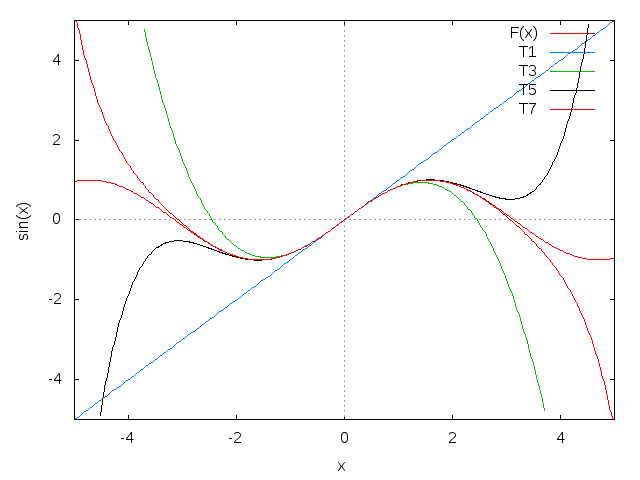
\includegraphics[width=10cm]{sen.png}
  \end{figure}
 
 
 
 \hspace {0.5cm}


 Desarrollo del teorema de Taylor de la función Log(1+x) de grado 4,7,11,16.
 \begin{verbatim}
 /* [wxMaxima batch file version 1] [ DO NOT EDIT BY HAND! ]*/
/* [ Created with http://maxima-online.org ] */


/* [wxMaxima: comment start ]
This solution online http://maxima-online.org/?inc=r467725079
   [wxMaxima: comment end   ] */


/* [wxMaxima: input   start ] */
f(x):=log(1+x);
taylor(f(x),x,0,4);
taylor(f(x),x,0,7);
taylor(f(x),x,0,11);
taylor(f(x),x,0,17);
fortran(taylor(f(x),x,0,4));
fortran(taylor(f(x),x,0,7));
fortran(taylor(f(x),x,0,11));
fortran(taylor(f(x),x,0,16));
tex(taylor(f(x),x,0,4));
tex(taylor(f(x),x,0,7));
tex(taylor(f(x),x,0,11));
tex(taylor(f(x),x,0,16));
plot2d([f(x),taylor(f(x),x,0,4),
taylor(f(x),x,0,7),
taylor(f(x),x,0,11),taylor(f(x),x,0,16)],
[x,-5,5],[y,-5,5],[color,red,blue,green,black],[legend,F(x),T4,T7,T11,T16],
   [ylabel,f(x)]);
/* [wxMaxima: input   end   ] */
 \end{verbatim}
 
  \begin{center}
  
    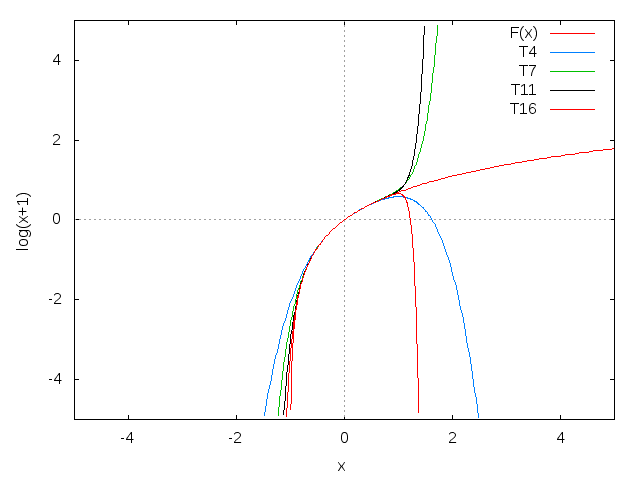
\includegraphics[width=10cm]{lod.png}
  \end{center}
 
 
 
 
 
 \hspace {0.5cm}
 
 
 Desarrollo del teorema de Taylor de la función Log(cos(x)) de grado 4,7,11,16
 \begin{verbatim}
 /* [wxMaxima batch file version 1] [ DO NOT EDIT BY HAND! ]*/
/* [ Created with http://maxima-online.org ] */


/* [wxMaxima: comment start ]
This solution online http://maxima-online.org/?inc=r-1963182626
   [wxMaxima: comment end   ] */


/* [wxMaxima: input   start ] */
f(x):=log(cos(x));
taylor(f(x),x,0,4);
taylor(f(x),x,0,7);
taylor(f(x),x,0,11);
taylor(f(x),x,0,16);
fortran(taylor(f(x),x,0,4));
 fortran(taylor(f(x),x,0,7));
fortran(taylor(f(x),x,0,11));
fortran(taylor(f(x),x,0,16));
tex(taylor(f(x),x,0,4));
tex(taylor(f(x),x,0,7));
tex(taylor(f(x),x,0,11));
tex(taylor(f(x),x,0,16));
plot2d([f(x),taylor(f(x),x,0,4),taylor(f(x),x,0,7),
taylor(f(x),x,0,11),taylor(f(x),x,0,16)],
 [x,-%pi/2,%pi/2],[y,-%pi/2,%pi/2],
 [color,red,blue,green,black],
 [legend,F(x),T4,T7,T11,T16]
 ,[ylabel,f(x)]);
/* [wxMaxima: input   end   ] */
 \end{verbatim}
 
 
 
   \begin{center}
  
    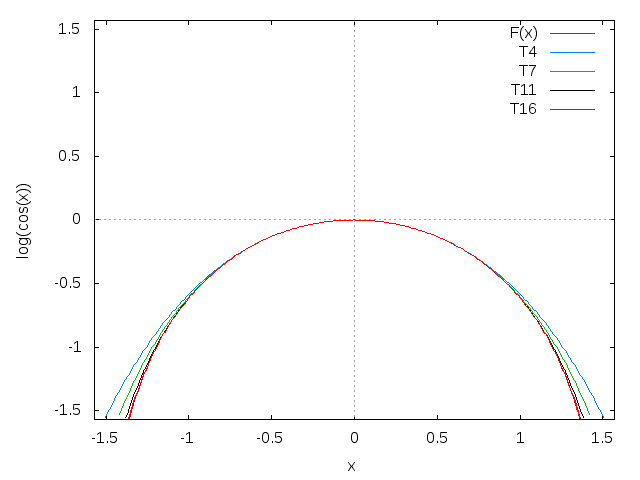
\includegraphics[width=10cm]{logcos.png}
  \end{center}
 
 
 \hspace {0.5cm}


 Desarrollo del teorema de Taylor de la función exp(x)/cos(x) de grado 2,4,11,18.
 \begin{verbatim}
 /* [wxMaxima batch file version 1] [ DO NOT EDIT BY HAND! ]*/
/* [ Created with http://maxima-online.org ] */


/* [wxMaxima: comment start ]
This solution online http://maxima-online.org/?inc=r-2094003024
   [wxMaxima: comment end   ] */


/* [wxMaxima: input   start ] */
f(x):=exp(x)/(cos(x));
taylor(f(x),x,0,2);
taylor(f(x),x,0,4);
taylor(f(x),x,0,11);
taylor(f(x),x,0,18);
fortran(taylor(f(x),x,0,2));
 fortran(taylor(f(x),x,0,4));
fortran(taylor(f(x),x,0,11));
fortran(taylor(f(x),x,0,18));
tex(taylor(f(x),x,0,2));
tex(taylor(f(x),x,0,4));
tex(taylor(f(x),x,0,11));
tex(taylor(f(x),x,0,18));
plot2d([f(x),taylor(f(x),x,0,2),
taylor(f(x),x,0,4),
taylor(f(x),x,0,11),taylor(f(x),x,0,18)]
 ,[x,-%pi/2,%pi/2],[y,-%pi/2,%pi/2],
 [color,red,blue,green,black],
 [legend,F(x),T2,T4,T11,T18],
 [ylabel,f(x)]);
/* [wxMaxima: input   end   ] */
 \end{verbatim}
 
 
   \begin{center}
  
    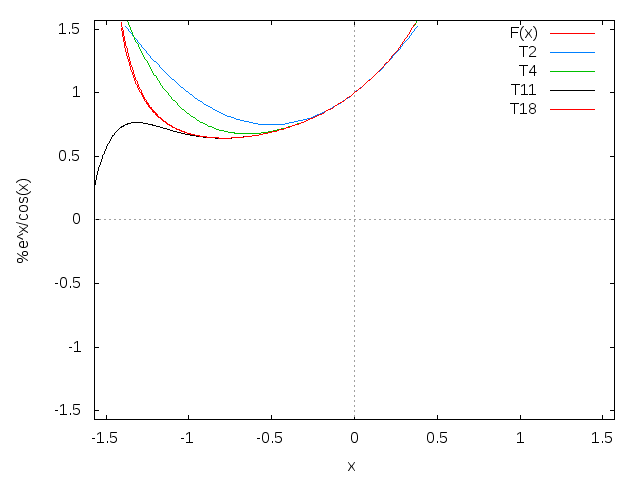
\includegraphics[width=10cm]{expcos.png}
  \end{center}
 
 
 \hspace {0.5cm}


  Desarrollo del teorema de Taylor de la función (1+x)*exp(x) de grado 4,7,11,16.
\begin{verbatim}
 /* [wxMaxima batch file version 1] [ DO NOT EDIT BY HAND! ]*/
/* [ Created with http://maxima-online.org ] */


/* [wxMaxima: comment start ]
This solution online http://maxima-online.org/?inc=r1077427305
   [wxMaxima: comment end   ] */


/* [wxMaxima: input   start ] */
f(x):=(1+x)*(exp(x));
taylor(f(x),x,0,4);
taylor(f(x),x,0,7);
taylor(f(x),x,0,11);
taylor(f(x),x,0,16);
fortran(taylor(f(x),x,0,4));
 fortran(taylor(f(x),x,0,7));
fortran(taylor(f(x),x,0,11));
fortran(taylor(f(x),x,0,16));
tex(taylor(f(x),x,0,4));
tex(taylor(f(x),x,0,7));
tex(taylor(f(x),x,0,11));
tex(taylor(f(x),x,0,16));
plot2d([f(x),taylor(f(x),x,0,4),taylor(f(x),x,0,7),
taylor(f(x),x,0,11),taylor(f(x),x,0,16)],
 [x,-%pi/2,%pi/2],[y,-%pi/2,%pi/2],
 [color,red,blue,green,black],
 [legend,F(x),T4,T7,T11,T16]
 ,[ylabel,f(x)]);
/* [wxMaxima: input   end   ] */
 \end{verbatim}
 
 
   \begin{center}
  
    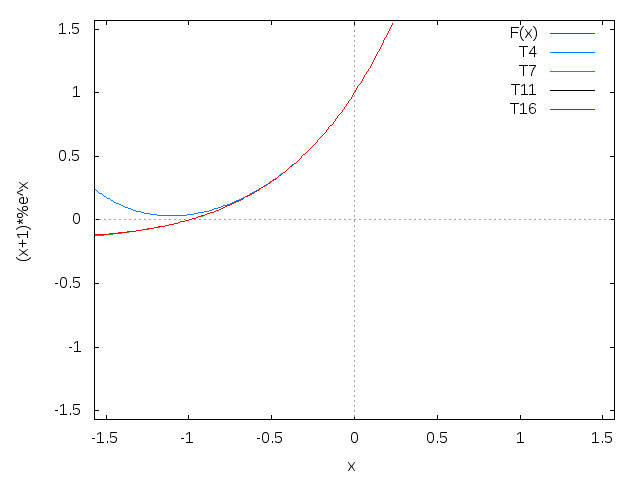
\includegraphics[width=10cm]{1xexp.png}
  \end{center}
 
 
 
 \hspace {0.5cm}

 
\end{document}

